\chapter{Evolutionäre Algorithmen}

Diese Subkategorie von Algorithmen wurde durch den natürlichen Prozess der Evolution
inspiriert. Charles Darwin begründete 1838 den Evolutionsprozess und das daraus resultierende
Überleben der jeweils am besten angepassten Individuen mit der natürlichen Selektion \cite{Wiki02}.
Diese stellt sicher, dass sich gut an den Lebensraum angepasst Lebewesen in der Natur
durchsetzen können, währenddessen weniger gut angepasste Individuen aussterben. Zudem
arbeitet die Natur nach dem 'Trial and Error' Prinzip. Dadurch werden Mutationen an
Lebewesen ausprobiert und bei positivem Effekt auf das Überleben der Spezies beibehalten,
bei einer Verminderung der Überlebenschancen jedoch wieder rückgängig gemacht. Dieser Prozess
ist sehr zeitaufwändig, jedoch nachhaltig wirksam. Viele Algorithmen wie beispielsweise
der Hill Climbing Algorithmus \cite{Anr18} wenden ebenfalls dieses Prinzip an.

\section{Genetische Algorithmen}

Die Genetischen Algorithmen sind die bekanntesten Vertreter aus der Gruppe der Evolutionären
Algorithmen. Sie orientierten sich an der Populationsgenetik und insbesondere an den Mendelschen
Regeln \cite{Mcc00}.
Bei Genetischen Algorithmen werden häufig Begriffe aus der Biologie verwendet. Die Anzahl an
möglichen Lösungen nennt man Population. Eine einzelne Lösungsvariante wird als Chromosom
bezeichnet, wohingegen diese wiederum aus einer Kombination an Variablen, in der Biologie Gene
genannt, bestehen. Wie aus der Grafik \ref{fig:genetics} zu entnehmen ist, besteht ein Chromosom
$A_n$ aus mehreren Genen.
\\
\begin{figure}[h!]
  \centering
  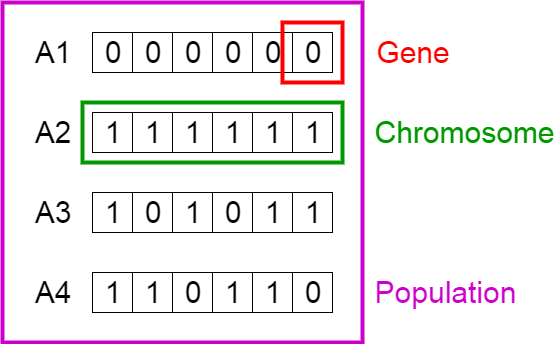
\includegraphics[scale=0.5]{resources/genetic_algorithms.png}
  \caption{Population, Chromosome und Gene \cite{Mal17}}
  \label{fig:genetics}
\end{figure}

\subsection{Funktionsweise}

Im folgenden werden die einzelnen Schritte erläutert, welche die Natur wie auch die Genetischen
Algorithmen durchlaufen, um eine Anfangspopulation schrittweise weiterzuentwickeln. Die Natur
sucht nach der erfolgsversprechendsten Lösung zum Überleben, wohingegen die Algorithmen
optimale Lösungen für ganz unterschiedliche Problemstellungen suchen. \cite{Mal17}

\subsubsection{Initiale Population}
Eine Population besteht aus mehreren unabhängigen Lösungen, im biologischen Kontext Chromosomen,
um eine bestimmte Problemstellung zu lösen. Bei den meisten Implementationen von Genetischen
Algorithmen wird ein Gen durch einen String repräsentiert. Bei Chromosomen eignen sich auch
Binärwerte um das Vorhandensein eines Gens auszuzeichnen.

\subsubsection{Selektion}
Anhand einer sogenannten Fitnessfunktion wird für jedes Individuum eine Punktzahl berechnet.
Die Punktzahl gibt darüber Auskunft, wie kompetitiv sich ein Individuum gegenüber einem anderen
verhält. Je höher dieser Wert, desto höher sind die Chancen, das besagtes Individuum von der
Selektion für die Reproduktion verwendet wird. Durch die Selektion können nur die fittesten
Individuen ihre Gene an die nächste Generation weitergeben und den schwächeren Individuen wird
der Reproduktionszyklus verwehrt.

\subsubsection{Kreuzung}
Der womöglich zentralste Bestandteil eines Genetischen Algorithmus ist die Kreuzung. Hier werden
aus den zuvor selektierten Individuen, einer Ansammlung der vielversprechendsten Lösungen, zwei
Individuen zur Paarung ausgewählt. Die beiden Ausgewählten tauschen ihre Gene bis zu einem bestimmten
Punkt, dem sogenannten Crossover Point, aus. Die restlichen Gene hinter diesem Punkt werden nicht
verändert. Durch diesen Prozess entstehen gleich zwei neue Individuen.

\subsubsection{Mutation}
Die Natur nutzt Mutationen aus, um die Artenvielfalt innerhalb einer Population zu gewährleisten.
Trotz der geringen Wahrscheinlichkeit kommt es vor, dass einzelne Gene, welche durch die Kreuzung
eigentlich vorhanden wären, nicht mehr vorhanden sind und umgekehrt. Ein Genetischer Algorithmus
flippt beispielsweise einzelne Variablen seiner Nachkommen. Durch die Mutation wird verhindert,
dass unser Algorithmus in einem lokalen Minimum stecken bleibt.

\subsubsection{Terminierung}
Ein Genetischer Algorithmus terminiert, sobald sich die nächste Generation nicht mehr merklich von
ihren Vorgängern unterscheidet. Man spricht oftmals auch von Konvergenz. Es ist jedem Algorithmus
selbst überlassen, wie lange ein Individuum in der Population überlebt. Häufig werden bei jedem
Reproduktionszyklus ein oder mehrere Individuen mit den niedrigsten Fitnesswerten aus der Population
gestrichen. In der Natur übernimmt der Tod diese Funktion.

\subsection{Beispiel Implementation}
Die einzelnen Schritte eines Genetischen Algorithmus sind in Listing A.1 durch
ein Python-Beispiel verdeutlicht. Die verwendete Fitnessfunktion ist sehr rudimentär
gehalten und berechnet lediglich die Summe der vorhandenen Gene. Die Population ist konvergiert,
wenn ein Individuum den Fitnesswert 5 erreicht, sprich alle Gene vorhanden sind.

Zweck dieses Listings ist es, den Ablauf eines Genetischen Algorithmus verständlich darzustellen.
Für eine bessere Übersicht wurden dazu uninteressante Teile des Codes gänzlich weggelassen.

\subsection{Vorteile}
Genetische Algorithmen haben gewisse Vorzüge bei der Lösung von komplexen
Problemstellungen gegenüber traditionellen Verfahren. Durch den modularen Aufbau
mit den drei Hauptfunktionen Selektion, Kreuzung und Mutation, lassen sich diese
Algorithmen einfach parallelisieren, was sich in einer besseren Rechenzeit bemerkbar
macht. Weiter generieren sie nicht nur eine Lösung sondern eine Vielzahl an möglichen
Lösungen, welche mit der Zeit immer bessere Ergebnisse liefern. \cite{Gou19}

\subsection{Anwendungsgebiete}
Es existieren schier endlose Einsatzmöglichkeiten für Genetische Algorithmen. Sie werden unter anderem
zum Trainieren von Neuronalen Netzwerken eingesetzt, zur Berechnung von Fahrplänen wie auch den zu fahrenden
Routen (analog dem Traveling Salesman Problem), zur Konstruktion von Aerodynamischen Fahrzeugchassis in
der Luftfahrts- sowie in der Automobilbranche und häufig auch in der Finanzwirtschaft wie beispielsweise
zur dynamischen Preisberechnung \cite{Tut}.

\section{Genetic Programming}
Eine weitere Unterart der Evolutionären Algorithmen ist Genetic Programming. Ähnlich wie
bei den Genetischen Algorithmen ist Genetic Programming auch von den Mendelschen Regeln
inspiriert worden. Die Population besteht jedoch nicht wie bisher gezeigt aus einzelnen
Lösungen, sondern aus Programmen, welche eine Aufgabenstellung in unterschiedlicher
Qualität lösen können. Ziel ist es, dass diese Programme durch den Vererbungsprozess
von Generation zu Generation besser auf die jeweilige Problemstellung angepasst werden.
\cite{GenGP}

\subsection{Darstellungsformen}
Es stellt sich die Frage, wie eine Applikation repräsentiert werden kann, um anschliessend von
Genetic Programming optimiert werden zu können. Es existieren nebst Tree- und Stack-basierten
eine Lineare sowie eine Kartesische Darstellungsform. Im folgenden wird die Tree-basierte Form
genauer erläutert.

\begin{figure}[h!]
  \centering
  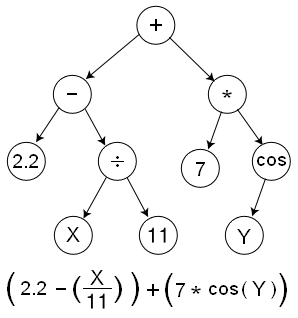
\includegraphics[scale=0.5]{resources/genetic_program_tree.png}
  \caption{Einfaches mathematisches Programm als Tree dargestellt \cite{Wiki01}}
  \label{fig:gp_tree}
\end{figure}

Wie in Grafik \ref{fig:gp_tree} erkennbar ist, werden die einzelnen Operationen in der Tree-basierten
Darstellungsweise durch Knoten repräsentiert. Die Operanden sind dabei jeweils die Endknoten.
Der Vorteil von einem Tree ist, dass mittels Rekursion sehr simpel über alle Äste iteriert werden
kann. Bei der Kreuzung innerhalb des Genetic Programming Algorithmus werden beispielsweise einzelne
Äste zweier Bäume miteinander kombiniert um einen komplett neuen Baum zu kreieren. \cite{GenTree}

\subsection{Anwendungsgebiete}
Genetic Programming wird häufig als Machine Learning Tool eingesetzt. Es ist besonders nützlich, wenn
eine Approximation der finalen Lösung genügt, da die Berechnung einer exakten Lösung zu aufwändig
wäre. Ausserdem hilft es in Fällen, wo die genaue Form der Lösung zu Beginn unbekannt ist. Häufige
Einsatzgebiete sind Data Modeling, Feature selection und Klassifikation.

Es existieren unzählige Beispiele, in denen mit Genetic Programming gleichwertige, wenn nicht sogar
bessere Ergebnisse erzielt wurden als durch einen Menschen. Das Entwerfen von elektrischen
Schaltplänen, KI in Computerspielen, Bilderkennung oder automatisiertes Bugfixing stellen nur einen
kleinen Teil der Einsatzmöglichkeiten dar. \cite{Koz10}


\section{Weitere Algorithmen}
Nebst den beiden behandelten Klassen von Genetischen Algorithmen und dem Genetic Programming existieren
noch weitere Unterarten von Evolutionären Algorithmen. Diese werden hier lediglich aufgelistet, da
eine detaillierte Differenzierung zu den beiden bereits bekannten Algorithmen aus dieser Gruppe den Rahmen
dieser Seminararbeit sprengen würde. Weitere Evolutionäre Algorithmen sind:

\begin{itemize}
  \item Evolution Strategies
  \item Grammatical Evolution
  \item Learning Classifier System
\end{itemize}